\pagebreak
\restoregeometry 
\section{Análisis por agrupación.}

Con el fin de identificar grupos con características similares de forma automática, se procedió a usar algoritmos de clustering. Específicamente, se hace clustering jerárquico completo usando la función \textsf{agnes} de la biblioteca \textsf{cluster}. 

\subsection{Elección del número de clusters}

Existen criterios para la elección de número de clusters adecuado dado un conjunto de datos, los criterios utilizados en este problema son dos:  suma de cuadrados entre clústers (wss) y el criterio de ancho de \textit{silhouette}.
En el primer caso, el criterio consiste en graficar la suma de cuadrados entre clústers para varios números de clústers y observar a partir de que número la mejora a la suma de cuadrados entre clústers es mínima. En una gráfica que compare a wss con el número de clusters, se espera que en el número óptimo se forme un \textit{codo} que indique el cumplimiento del criterio. La figura \ref{i_cluster_Elbow} muestra el resultado de calcular wss para ciertos números de clústers. A partir de observar la gráfica, se determina que una cantidad adecuada para el número de clusters usando estre criterio es $5$.


\begin{figure}[h]
\centering
	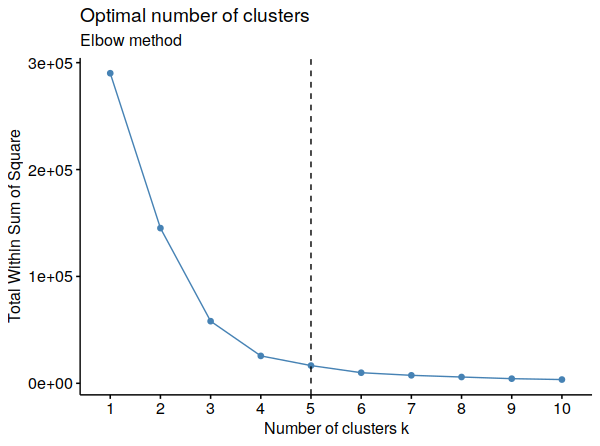
\includegraphics[scale=.5]{images/clusterElbow.png} 
	\label{i_cluster_Elbow}
	\caption{Suma total de cuadrados entre clústers vs número de clusters}
\end{figure}


El otro criterio muy popular en la literatura es el método silhouette, que es una medida de qué tan bien un individuo está asignado en un clúster a partir de calcular la distancia promedio a cada uno de los elementos del clúster al que fue asignado y la distancia promedio al clúster más cercano de entre aquellos a los que no pertenece. Mientras más alta sea la medida promedio silhouette, mejor asignados están los datos en sus respectivos clústers. La figura \ref{i_cluster_Silhouette} muestra la comparativa de ancho de silhouette promedio para cierto número de clústers, y se observa que el número adecuado de clústers para los datos es $5$. Para la creación de las gráficas de wss y silhouette se usó la función \textsf{fviz\_nbclust} de la biblioteca factoextra.


\begin{figure}[h]
\centering
	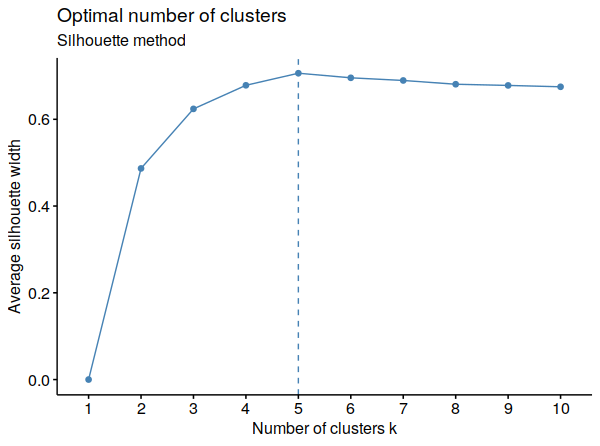
\includegraphics[scale=.5]{images/clusterSilhouette.png} 
	\label{i_cluster_Silhouette}
	\caption{Silhouette promedio vs número de clusters}
\end{figure}

\pagebreak
\subsection{Asignación de clusters}

Habiendo elegido el número de clústers por crear, se procedió a calcular la asignación de los datos a cada clúster, usando clustering jerárquico con la ayuda de la función \textsf{agnes}. Los clústers obtenidos se muestran en las representaciones en dos dimensiones de los datos (PCA y Factores) en las figuras \ref{i_cluster_PCA} y \ref{i_cluster_Factores}. En ambos casos se observa que los grupos formados coinciden con los descritos en la sección de reducción de dimensión. Hay que notar que cada una de las marcas de pizza está contenida en un único clúster.

\begin{figure}[h]
\centering
	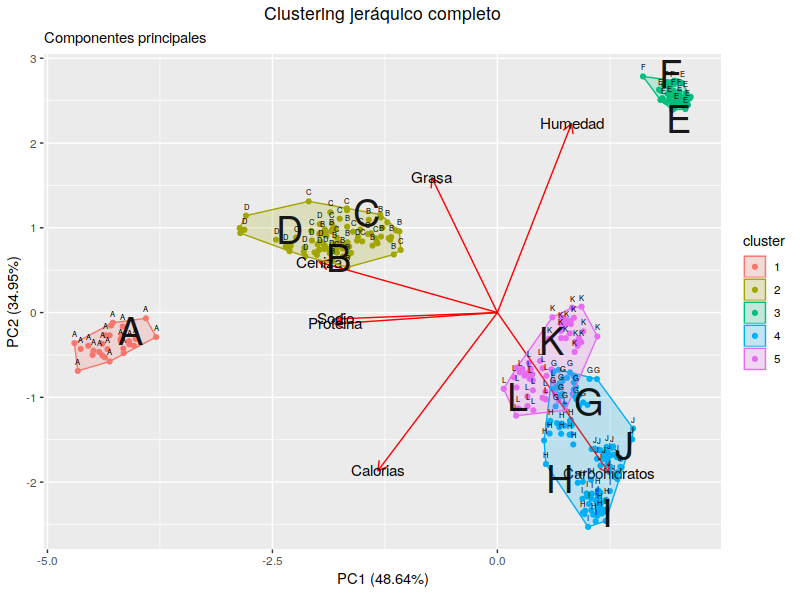
\includegraphics[scale=.75]{images/clusterPCA.png} 
	\label{i_cluster_PCA}
	\caption{Clustering jerárquico completo (Representación: PCA)}
\end{figure}


\begin{figure}[h]
\centering
	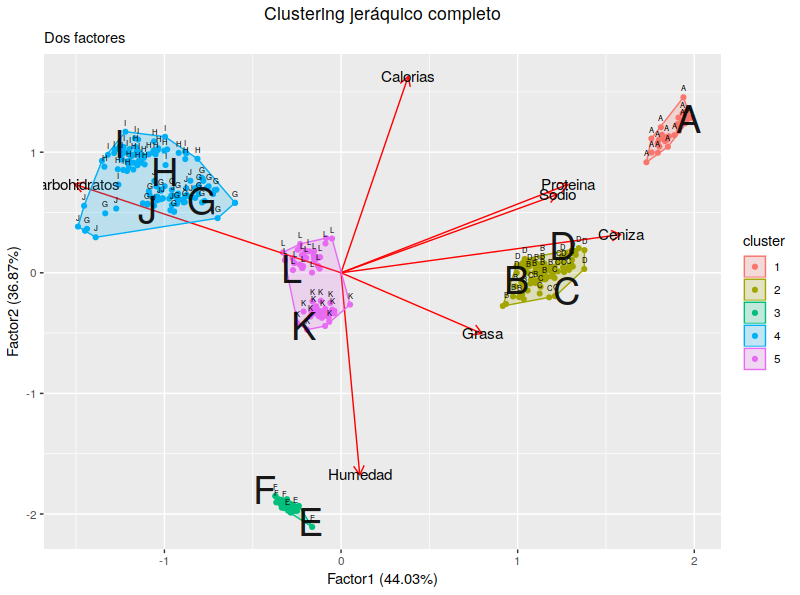
\includegraphics[scale=.75]{images/clusterFactores.png} 
	\label{i_cluster_Factores}
	\caption{Clustering jerárquico completo (Representación: Factores)}
\end{figure}